\documentclass[11pt]{article}
\usepackage[utf8]{inputenc} % Para caracteres en espa�ol
\usepackage{amsmath,amsthm,amsfonts,amssymb,amscd}
\usepackage{multirow,booktabs}
\usepackage[table]{xcolor}
\usepackage{fullpage}
\usepackage{lastpage}
\usepackage{enumitem}
\usepackage{multicol}
\usepackage{fancyhdr}
\usepackage{mathrsfs}
\usepackage{pdfpages}
\usepackage{wrapfig}
\usepackage{setspace}
\usepackage{esvect}
\usepackage{calc}
\usepackage{multicol}
\usepackage{cancel}
\usepackage{graphicx}
\graphicspath{ {pictures/} }
\usepackage[retainorgcmds]{IEEEtrantools}
\usepackage[margin=3cm]{geometry}
\usepackage{amsmath}
\newlength{\tabcont}
\setlength{\parindent}{0.0in}
\setlength{\parskip}{0.05in}
\usepackage{empheq}
\usepackage{framed}
\usepackage[most]{tcolorbox}
\usepackage{xcolor}
\colorlet{shadecolor}{orange!15}
\parindent 0in
\parskip 12pt
\geometry{margin=1in, headsep=0.25in}
\theoremstyle{definition}
\newtheorem{defn}{Definition}
\newtheorem{reg}{Rule}
\newtheorem{exer}{Exercise}

% Two more packages that make it easy to show MATLAB code
\usepackage[T1]{fontenc}
\usepackage[framed,numbered]{matlab-prettifier}
\lstset{
	style = Matlab-editor,
	basicstyle=\mlttfamily\small,
}

\newtheorem{note}{Note}
\begin{document}
\setcounter{section}{0}

\thispagestyle{empty}

\begin{center}
{\LARGE \bf Homework 2 Problem 8}\\
{\large AE403 - Spring 2018 \\ Emilio R. Gordon}
\end{center}
\vspace{20mm}
The plots required for part A and part B are shown in the following pages.  The initial conditions for this problem were defined to be
\begin{itemize}
\item \textbf{Initial Rotation Matrix}
\begin{equation*}
\begin{aligned}
\begin{bmatrix}
1 & 0 & 0 \\ 0 & 1 & 0 \\ 0 & 0 & 1
\end{bmatrix}
\end{aligned}
\end{equation*}
\item \textbf{Initial Euler Angles}
\begin{equation*}
\begin{aligned}
\begin{bmatrix}
0 \\ 0 \\ 0
\end{bmatrix}
\end{aligned}
\end{equation*}
\item \textbf{Initial Quaternion}
\begin{equation*}
\begin{aligned}
Q = (q_o , q) = \Bigg( 0, 
\begin{bmatrix}
0 \\ 0 \\ 1
\end{bmatrix} \Bigg)
\end{aligned}
\end{equation*}
\end{itemize}
A function begins by defining a time interval which we are saying is 6 seconds. After which, we define the Initial conditions as mentioned above. After which ODE45 is utilized to generate the state values of Rotation matrix, Euler Angles and Quaternions.
\begin{figure}[h!]
\begin{lstlisting}
% DEFINE THE TIME INTERVAL
tMax = 6;
tRate = 30;
t = linspace(0,tMax,tMax*tRate);

%DEFINE THE INITIAL CONDITIONS
xH0 = [0;0;0];
R0 = eye(3);
xQ0 = [0; 0; 0; 1];

% INTEGRATE THE ANGULAR RATE EQUATIONS
[t,xR] = ode45(@fR,t,RtoX(R0));
[t,xH] = ode45(@fH,t,xH0);
[t,xQ] = ode45(@fQ,t,xQ0);
\end{lstlisting}
\caption{ODE45 and Setup}
\end{figure}
\newpage
After ODE45 has completed, the final states can be gathered by the following script.
\newline
\begin{figure}[h!]
\begin{lstlisting}
%Collect State at t=6 seconds
finalR = xR(end,:)
finalH = xH(end,:)
finalQ = xQ(end,:)
\end{lstlisting}
\caption{State at t=6 seconds}
\end{figure}
\newline
From this, it appears that:
\newline
\begin{itemize}
\item \textbf{Rotation Matrix at 6 Seconds}
\begin{equation*}
\begin{aligned}
\begin{bmatrix}
-0.3524  &  0.7206 &  -0.5971 \\
   -0.2036 &  -0.6817  & -0.7027 \\
   -0.9135  & -0.1261  &  0.3869 \\
\end{bmatrix}
\end{aligned}
\end{equation*}
\item \textbf{Euler Angles at 6 Seconds}
\begin{equation*}
\begin{aligned}
\begin{bmatrix}
1.0657 \\
   -0.6396 \\
    4.2568 \\
\end{bmatrix}
\end{aligned}
\end{equation*}
\item \textbf{Quaternion at 6 Seconds}
\begin{equation*}
\begin{aligned}
Q = (q_o , q) = \Bigg( -0.7783 , 
\begin{bmatrix}
0.2667 \\
   -0.4854 \\
   -0.2973 \\
\end{bmatrix} \Bigg) 
\end{aligned}
\end{equation*}
\end{itemize}
\newline
Which only partially answers part c. 
\newpage
Part C further ask to convert our final Euler Angles and Quaternion into a rotation matrix. This can easily be done in Matlab as shown in Figure 3.
\newline
\begin{figure}[h!]
\begin{lstlisting}
% CODE TO CONVERT FROM XYZ EULER ANGLES TO A ROTATION MATRIX
function R=HtoR(H)
	theta1 = H(1);
	theta2 = H(2);
	theta3 = H(3);

	R11 = cos(theta2)*cos(theta3);
	R12 = -cos(theta2)*sin(theta3);
	R13 = sin(theta2);

	R21 = sin(theta1)*sin(theta2)*cos(theta3)+cos(theta1)*sin(theta3);
	R22 = -sin(theta1)*sin(theta2)*sin(theta3)+cos(theta1)*cos(theta3);
	R23 = -sin(theta1)*cos(theta2);

	R31 = -cos(theta1)*sin(theta2)*cos(theta3)+sin(theta1)*sin(theta3);
	R32 = cos(theta1)*sin(theta2)*sin(theta3)+sin(theta1)*cos(theta3);
	R33 = cos(theta1)*cos(theta2);

R=[R11 R12 R13; R21 R22 R23; R31 R32 R33];

% CODE TO CONVERT FROM A QUATERNION TO A ROTATION MATRIX
function R=QtoR(q0,q)
	qhat = [0 -q(3) q(2); q(3) 0 -q(1); -q(2) q(1) 0];

R = (q0^2 - q'*q)*eye(3)+2*q*q'+2*q0*qhat;
\end{lstlisting}
\caption{Functions for Conversions}
\end{figure}
\newline
This provides the solution:
\newline
\begin{itemize}
\item \textbf{Rotation Matrix at 6 Seconds}
\begin{equation*}
\begin{aligned}
\begin{bmatrix}
-0.3524  &  0.7206 &  -0.5971 \\
   -0.2036 &  -0.6817  & -0.7027 \\
   -0.9135  & -0.1261  &  0.3869 \\
\end{bmatrix}
\end{aligned}
\end{equation*}
\item \textbf{Rotation Matrix from Euler Angles at 6 Seconds}
\begin{equation*}
\begin{aligned}
\begin{bmatrix}
-0.3530  &  0.7205  & -0.5968 \\
   -0.2047  & -0.6819 &  -0.7022 \\
   -0.9129  & -0.1257 &   0.3883 \\
\end{bmatrix}
\end{aligned}
\end{equation*}
\item \textbf{Rotation Matrix from  Quaternion at 6 Seconds}
\begin{equation*}
\begin{aligned}
\begin{bmatrix}
0.3529  & -0.7216  &  0.5971 \\
    0.2038   & 0.6819  &  0.7037 \\
   -0.9142 &  -0.1265  &  0.3874 \\
\end{bmatrix}
\end{aligned}
\end{equation*}
\end{itemize}
\newpage
The rotation matrices derived from each coordinate system resulted in relatively the same matrix. That said, there is some error due to numerical rounding. This confirms our earlier analysis and work since, regardless of approach, we arrived at the same matrix.  One notable difference from our other set of initial conditions is how the quaternion still match in magnitude but sometimes differs in the sign produced.
\newline
\newline
Every approach has its pros and cons as follows:
\begin{center}
 \begin{tabular}{||c | c | c||} 
 \hline
 Name & Pros & Cons \\ [0.5ex] 
 \hline\hline
 Rotation Matrix & Always provides information on the state & Computational heavy \\
 & No singularity & 9 different elements to keep track of \\
 & & Not intuitive (opinion)\\ 
  \hline
 Euler Angles & Only 3 elements to work with.  & Singularity or "Gimbal Lock" \\
 & Computationally efficient & \\
& Intuitive (opinion) & \\
 \hline
 Quaternion & Computationally inexpensive & As seen in problem 7d, changing\\
 & Only 4 elements to work with & reference frames is computationally\\
 & No singularity & heavy\\
 & Intuitive (opinion) & \\ [1ex] 
 \hline
\end{tabular}
\end{center}
\newline
\vspace{20mm}
\newline
Plotting the states over time, the plots on the following page are produced. Notice how the states tend to reach a slope of zero towards the end. This tells us that the spacecraft is reaching a stable orientation. For complete code, please check compass.
\newpage
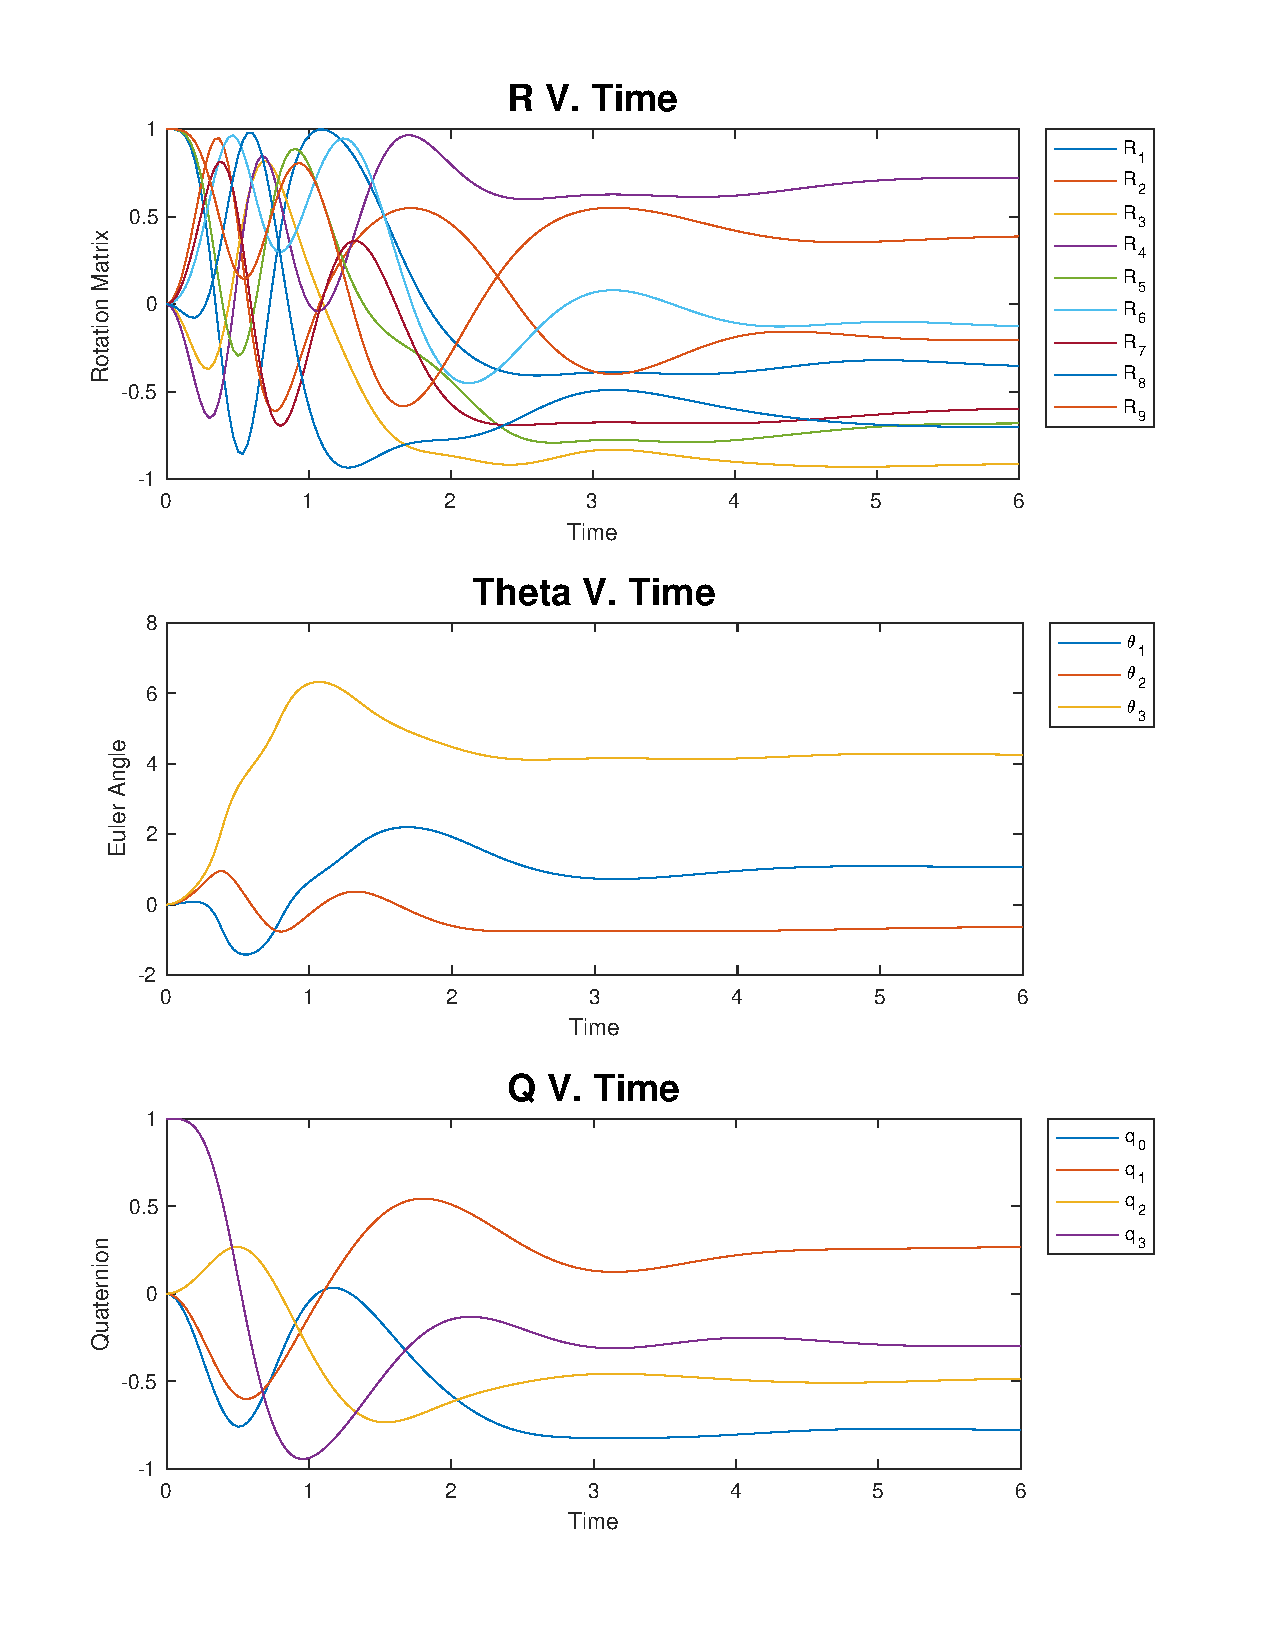
\includepdf{figure3.pdf} 
\newpage
Finally, another important part of this code is plotting the rates of change as asked in part b. This was done as shown below in Figure 4.
\newline
\begin{figure}[h!]
\begin{lstlisting}
% FIND THE RATES
for i=1:length(t)
    rdot(:,i) = RtoX(getRdot(t(i),XtoR(xR(i,:)')));
    thetadot(:,i) = getHdot(t(i),xH(i,:)');
    [q0dot(i),qdot(:,i)] = getQdot(t(i),xQ(i,1),xQ(i,2:4)');
end

function [q0dot, qdot] = getQdot(t,q0,q)
% CODE TO COMPUTE Qdot = (q0dot,qdot)
omega = 10*exp(-t)*[sin(t);sin(2*t);sin(3*t)];
omegahat = [0 -omega(3) omega(2);...
            omega(3) 0 -omega(1);...
           -omega(2) omega(1) 0];
       
q0dot = -0.5*omega'*q;
qdot = 0.5*(omega*q0 - omegahat*q);

function thetadot = getHdot(t,theta)
% CODE TO COMPUTE Thetadot
theta2 = theta(2);
theta3 = theta(3);
omega = 10*exp(-t)*[sin(t);sin(2*t);sin(3*t)];

B=[(cos(theta3)/cos(theta2)) (-sin(theta3)/cos(theta2)) 0;...
    (sin(theta3)) (cos(theta3)) 0;...
    (-tan(theta2)*cos(theta3)) (tan(theta2)*sin(theta3)) 1];

thetadot = B*omega;

function Rdot = getRdot(t,R)
% CODE TO COMPUTE Rdot
omega = 10*exp(-t)*[sin(t);sin(2*t);sin(3*t)];
omegahat = [0 -omega(3) omega(2); omega(3) 0 -omega(1); -omega(2) omega(1) 0];

Rdot = R*omegahat;
\end{lstlisting}
\caption{Functions Rates of Change}
\end{figure}
\newline
Running the function, the plots on the next page are produced. Note how the rates of change converge to zero as the simulation approaches 6 seconds.
\newpage
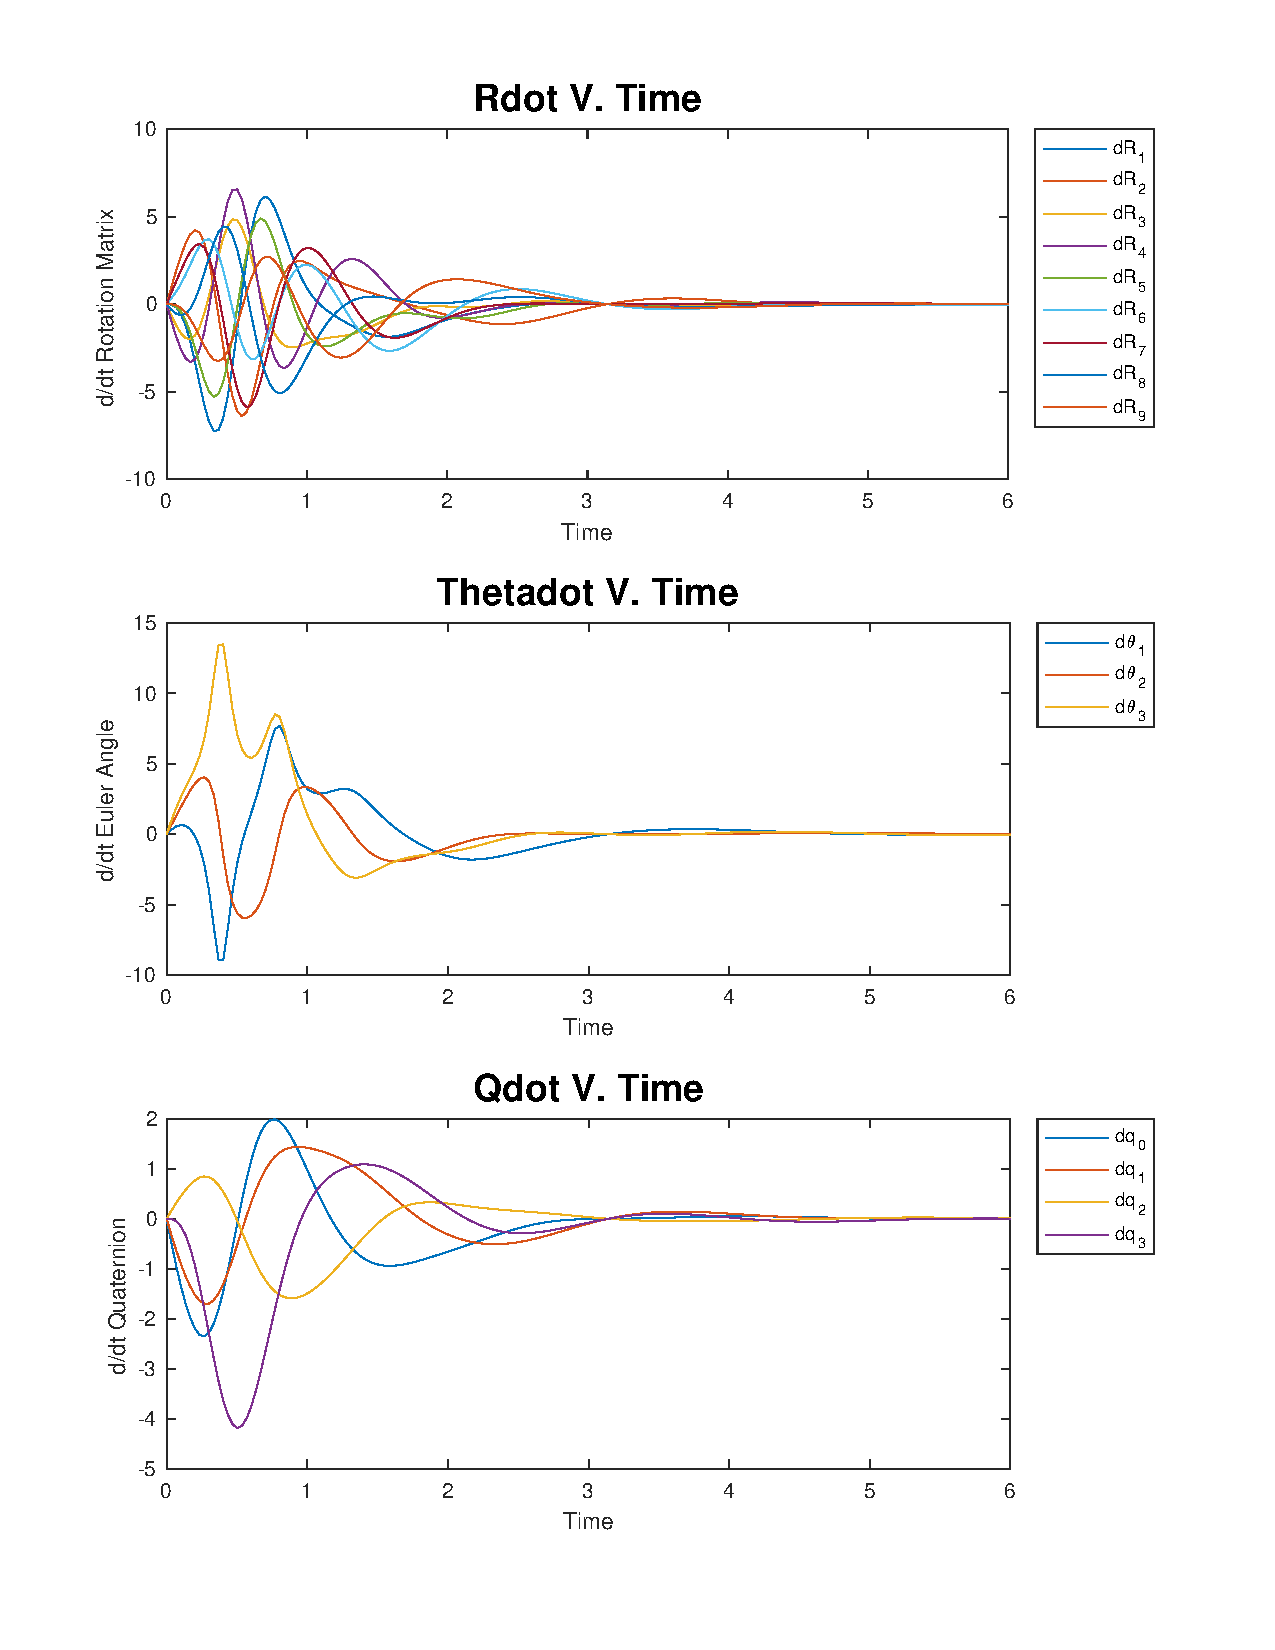
\includepdf{figure1.pdf} 
\end{document}